\documentclass[titlepage, 10pt]{ltjsarticle}
\usepackage[utf8]{inputenc}
\usepackage{graphicx, color, xcolor}
\usepackage{ascmac}
\usepackage{float}
\usepackage{enumitem}
\usepackage{tabularray}
\usepackage{listings, jvlisting}
\usepackage{amssymb}
\usepackage{wrapfig}
\usepackage{diagbox}
\usepackage{siunitx}
\usepackage{enshuc}

\title{情報科学演習C \\ 課題3} 
\author{植村 向陽}
\studentid{09B24008}
\affiliation{基礎工学部情報科学科ソフトウェア科学コース}
\date{\today} 

\begin{document}

\maketitle 

\textcolor{blue}{各課題について，実行結果（terminalの出力結果を記載すること）とその説明，動作をわかりやすく解説すること．その際，付録に載せたソースコードの行番号を適宜参照しながら説明すること．}

\section{課題3-1}
\subsection{実装方針・アルゴリズム}
親プロセスではファイル\texttt{counter}に対するセマフォを作成し，\texttt{fork()}を用いて\texttt{NUMPROCS}個の子プロセスを生成する．子プロセスはセマフォを用いて\texttt{counter}が利用できる状態になるのを待ち，利用できるようになるとセマフォを1減算してファイルをロックする．ロックした後，ファイル\texttt{counter}を開いて現在の値を読み取り，1加算してから書き戻す．この読み込みと書き込みの操作はクリティカルセクションであるため連続して実行される必要がある．最後にセマフォを1加算してファイル\texttt{counter}のロックを解除する．親プロセスは全ての子プロセスが終了するのを待ち，最後にファイル\texttt{counter}の値を読み取って出力する．なおセマフォの獲得の際\texttt{key}として\texttt{IPC\_PRIVATE}を用いた．これを行うと親プロセスと子プロセスのみが同じセマフォを共有することができる．
\subsection{実行結果}
\begin{figure}[H]
    \centering
    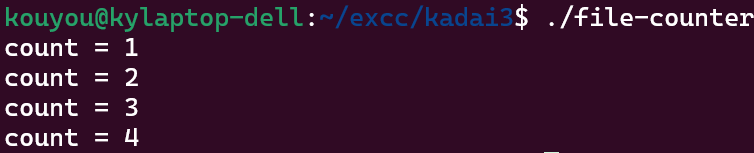
\includegraphics[scale = 0.7]{counter4.png}
    \caption{NUMPROCSを4に設定して実行した結果}
    \label{fig:counter4}
\end{figure}
\begin{figure}[H]
    \centering
    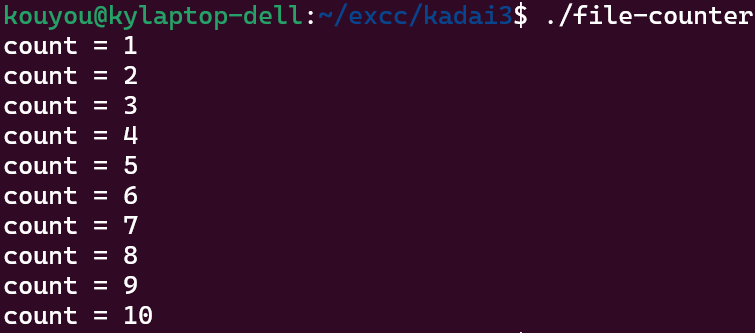
\includegraphics[scale = 0.7]{counter10.png}
    \caption{NUMPROCSを10に設定して実行した結果}
    \label{fig:counter10}
\end{figure}
NUMPROCSを4または10に設定し，\texttt{file-counter}を複数回実行したところ，いずれの実行も上図\ref{fig:counter4},\ref{fig:counter10}と同じ結果になった．このことから排他制御が正しく行われ，NUMPROCSの値に応じてファイル\texttt{counter}の値が正しく更新されていることがわかる．

\subsection{考察}
セマフォを用いない場合だと各子プロセスの読み取りと書き込みの順が不定になるため，ファイル\texttt{counter}の値が正しく更新されない場合があった．しかし，セマフォを用いることでファイル\texttt{counter}へのアクセスを1プロセスずつに制限し，読み書きの実行順を制御することができることが分かった．
\section{課題3-2-1}
\subsection{実装方針・アルゴリズム}
まず親プロセス内で親から子へのパイプと子から親へのパイプを作成する．次に\texttt{fork()}を用いて子プロセスを生成する．その後親と子はそれぞれパイプに対して不要なファイルディスクリプタを閉じ，パイプにメッセージを送信した後パイプからのメッセージを待機する．親プロセスは子プロセスからのメッセージを受信して出力し，子プロセスは親プロセスからのメッセージを受信して出力する．
\subsection{実行結果}
\begin{figure}[H]
    \centering
    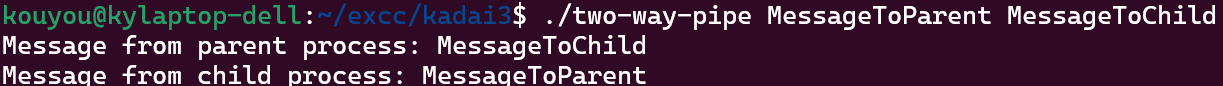
\includegraphics[scale = 0.45]{twowaypipe.png}
    \caption{双方向パイプの実行結果}
    \label{fig:twowaypipe}
\end{figure}
親と子の両方から正しくメッセージが出力されていることがわかる．このことから，双方向パイプを用いて親プロセスと子プロセスの間で正しく通信が行われていることがわかる．
\subsection{考察}

\section{課題3-2-2}
\subsection{実装方針・アルゴリズム}
親プロセスで配列の左半分，子プロセスで右半分をマージソートし，子は右半分のソート結果をパイプで親プロセスに送信する．プロセス分岐の際，メモリ領域が子プロセスにコピーされるため，親プロセスと子プロセスは同じ中身の配列をそれぞれ保持することできる．
親へのソート結果の送信の際，ポインタを用いることで親の配列の右半分に直接子のソート結果を書き込むことができる．親プロセスは子プロセスからのソート結果を受信してから、配列全体をマージしてソートする．
\subsection{実行結果}
\begin{figure}[H]
\begin{minipage}[b]{0.45\textwidth}
    \centering
    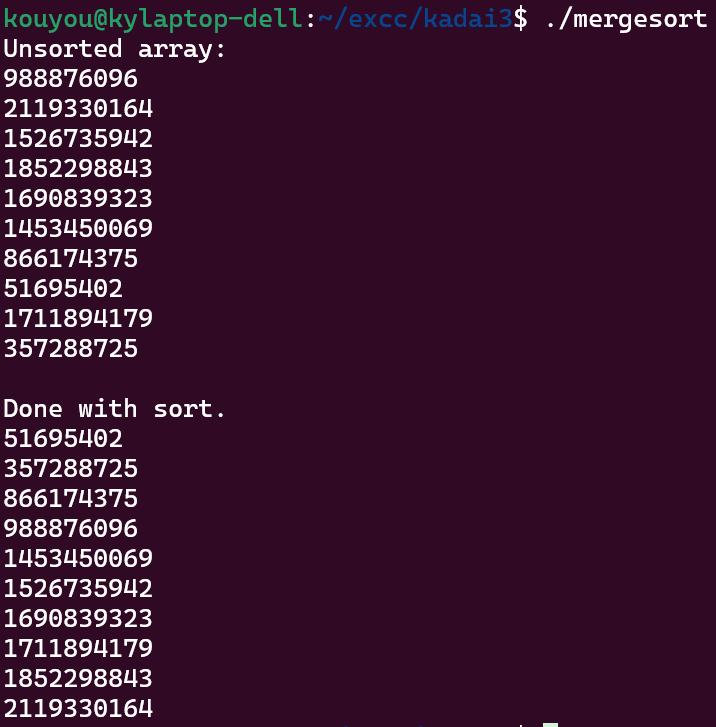
\includegraphics[width = 0.9\textwidth]{mergesort1.png}
    \label{fig:mergesort1}
\end{minipage}
\begin{minipage}[b]{0.45\textwidth}
    \centering
    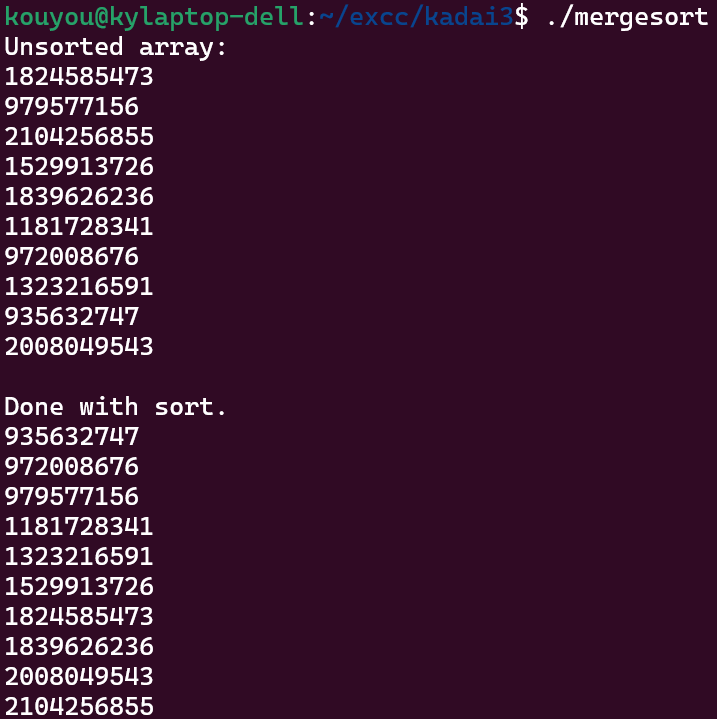
\includegraphics[width = 0.9\textwidth]{mergesort2.png}
    \label{fig:mergesort2}
\end{minipage}
\caption{マージソートの実行結果}
\end{figure}
上図\ref{fig:mergesort1}から異なる配列について正しくソートできていることがわかる．
\subsection{考察}
マージソートを2プロセスに分けて行う場合，ソートのみにかかる時間は少なくなると考えられる．しかし，実際にはプロセスの生成やパイプを用いた通信にかかるオーバーヘッドが存在するため，単純にプログラムの実行時間が半分になるとは限らず，むしろ実行時間が増加する可能性もある．特に、ソートする配列のサイズが小さい場合は、プロセスの生成や通信のオーバーヘッドがソートの時間よりも大きくなってしまう可能性がある．一方で、ソートする配列のサイズが大きい場合は、プロセスの生成や通信のオーバーヘッドが相対的に小さくなり、ソートの時間を短縮できる可能性がある．

\section{課題3-3-1}
\subsection{実装方針・アルゴリズム}
\text{myalarm}内では，まず\texttt{alarm}\texttt{signal()}を用いて\texttt{SIGCHLD}シグナルを無視するように設定する．これにより子プロセスを\texttt{wait()}する必要がなくなり、ゾンビプロセス化を回避できる．
次に\texttt{fork()}を用いて子プロセスを生成し，静的変数に子プロセスのPIDを保存する．関数内で静的変数を用いることで関数が終了しても値が保持され，変数の参照も関数内からのみ行えるため比較的安全である．この変数に前の子プロセスのPIDが保存されている場合は、そのPIDを\texttt{kill()}して前の子プロセスを終了させる．生成された子プロセスは\texttt{sleep()}で一定時間待機し，最後に\texttt{SIGALRM}シグナルを親プロセスに送信する．

親プロセスでは標準入力から文字列を読み取るたびに\text{myalarm}を呼び出す．これにより、前の子プロセスが存在する場合は終了させてから新しい子プロセスを生成し，タイムアウトのalarmを延長することができる．
\subsection{実行結果}
\begin{figure}[H]
    \centering
    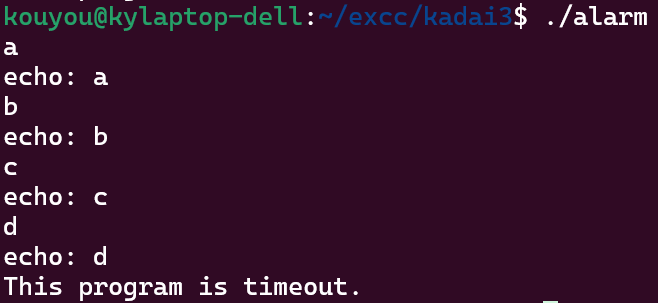
\includegraphics[scale = 0.6]{alarm-input.png}
    \caption{alarmへの入力}
    \label{fig:alarm-input}
\end{figure}
\begin{figure}[H]
    \centering
    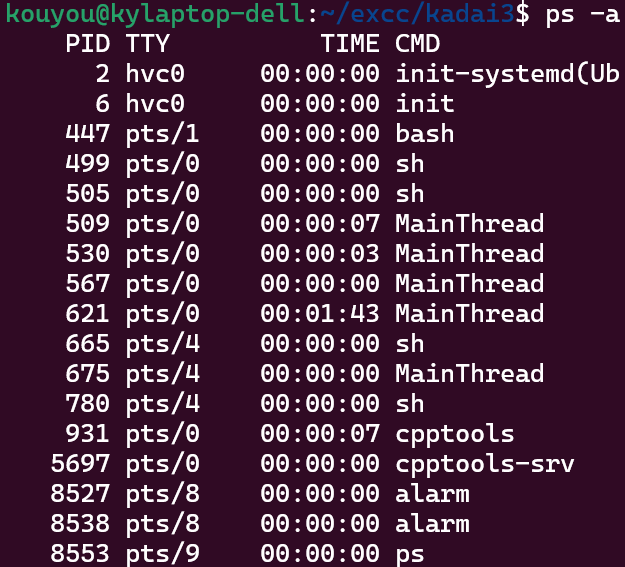
\includegraphics[scale = 0.6]{alarm-ps.png}
    \caption{alarmの子プロセスの状態をpsコマンドで確認した結果}
    \label{fig:alarm-ps}
\end{figure}
\texttt{alarm.c}をコンパイルして実行し、上図\ref{fig:alarm-input}のように標準入力から文字列を入力したところ，最後の入力から指定した秒数の後にシグナルが送信されプロセスが終了した．また、\texttt{ps}コマンドで子プロセスの状態を確認したところ，上図\ref{fig:alarm-ps}のように入力回数に関わらず\texttt{alarm}という名前のプロセスが2つ存在していることがわかった．つまり，親プロセスと子プロセスがそれぞれ1つずつ存在している．このことから、前の子プロセスを終了させてから新しい子プロセスを生成することで、ゾンビプロセス化を回避できていることがわかる．
\subsection{考察}
今回は\texttt{SIGCHLD}シグナルを無視することでゾンビプロセス化を回避したが，別の方法が無いか調べたところ\texttt{sigaction}関数を用いてシグナルハンドラを設定する方法があることが分かった．この方法では、子プロセスが終了したときにシグナルハンドラが呼び出され、その中で\texttt{wait()}を用いて子プロセスの終了を待機することでゾンビプロセス化を回避できる．

\section{課題3-3-2}
\subsection{実装方針・アルゴリズム}
まず\texttt{SIGALRM}に対するシグナルハンドラとして\texttt{timeout}関数を登録する．この関数内ではタイムアウトのフラグを立てる処理のみを行う．
サーバーに接続されると\texttt{myalarm}を呼び出し，タイマーをセットする．\texttt{select}によりサーバーからの応答または標準入力への書き込みを検知した場合は再度\texttt{myalarm}を呼び出してタイマーをリセットする．
\texttt{SIGALRM}が発生してタイムアウトのフラグが立てられた場合は、ソケットを閉じてからプログラムを終了する.

\subsection{実行結果}

\subsection{考察}



\section{発展課題}
\subsection{発展課題1}

\section{感想，意見，疑問等}


\appendix
\section{プログラム}
\subsection{課題3-1}
\subsection{課題3-2-1}
\subsection{課題3-2-2}
\subsection{課題3-3-1}
\subsection{課題3-3-2}
\subsection{発展課題}



\end{document}
